%% main_report51.tex
%% SAMBP TR-51/2026: Automatic Protection Settings Optimisation
%%
%% pdflatex main_report51.tex

\documentclass[11pt,a4paper]{article}

\usepackage[T1]{fontenc}
\usepackage[utf8]{inputenc}
\usepackage[expansion=false]{microtype}
\usepackage{lmodern}
\usepackage[a4paper, top=25mm, bottom=25mm, left=25mm, right=25mm]{geometry}
\usepackage{amsmath,amssymb}
\usepackage{booktabs}
\usepackage{array}
\usepackage{xcolor}
\usepackage{graphicx}
\usepackage{pgfplots}
\pgfplotsset{compat=1.18}
\usepackage{tikz}
\usetikzlibrary{arrows.meta,shapes.geometric,positioning,decorations.pathreplacing}
\usepackage{hyperref}
\usepackage[numbers,sort&compress]{natbib}

\definecolor{sambpblue}{RGB}{0,70,140}

\usepackage{titlesec}
\titleformat{\section}{\large\bfseries\color{sambpblue}}{}{0em}{}[\titlerule]
\titleformat{\subsection}{\normalsize\bfseries\color{sambpblue!80}}{}{0em}{}

\usepackage{fancyhdr}
\pagestyle{fancy}
\fancyhf{}
\rhead{\small\color{gray} SAMBP TR-51/2026}
\lhead{\small\color{gray} Automatic Protection Settings Optimisation}
\cfoot{\small\thepage}

\begin{document}

\begin{center}
  {\LARGE\bfseries\color{sambpblue} SAMBP Technical Report TR-51/2026}\\[6pt]
  {\large Automatic Protection Settings Optimisation}\\[10pt]
  {\normalsize PhD Thesis Supporting Report \quad|\quad 2026}
\end{center}

\vspace{2pt}\hrule\vspace{8pt}

\begin{abstract}
\noindent
This report develops an automatic relay settings engine for the 10-bus
SAMBP test network from TR-50.  The engine computes IEC Standard Inverse
pickup currents ($I_p$) and time-multiplier settings (TMS) for all 11
relays subject to sensitivity ($I_\mathrm{fault}>1.2\,I_p$ at 80\%
reach), coordination ($\mathrm{CTI}\geq200$\,ms) and range
($\mathrm{TMS}\in[0.05, 1.20]$) constraints.  Study C produces a
violation-free setting table (0 CTI violations) with TMS values graded
from 0.050 at the network extremities to 0.281 at the grid infeed relay
R01.  Study D shows that an IBR fleet change from $k_\mathrm{ibr}=0.35$
to $k_\mathrm{ibr}=0.60$ (16.7\,pp fault current increase per relay)
requires TMS updates on 6/11 relays with no $I_p$ changes, confirming
that the CUSUM-triggered WAPC retraining protocol from TR-48/TR-50 can
be extended to automatic setting re-dispatch with minimal relay
reconfiguration.  Study E demonstrates 100\% CTI pass rate on all 10
coordination pairs under $\pm10\%$ line impedance uncertainty
($N=500$\,trials), with minimum CTI across all pairs of 0.211\,s ---
above the 0.200\,s threshold with 5.5\% margin.
\end{abstract}

\vspace{4pt}\hrule\vspace{10pt}

% ─────────────────────────────────────────────────────────────────────────────
\section{Setting Constraints and Grading Method}
\label{sec:method}

Three constraints govern the setting engine:

\begin{center}
\begin{tabular}{@{}lll@{}}
\toprule
Constraint & Formula & Requirement \\
\midrule
Sensitivity & $I_\mathrm{fault}(0.8\,Z_L) \geq 1.2\,I_p$ & Relay operates for 80\%-reach fault \\
Coordination & $t_\mathrm{backup} - t_\mathrm{primary} \geq 200$\,ms & IEC\,60255-151 CTI \\
Range & $\mathrm{TMS} \in [0.050, 1.200]$ & IED hardware limits \\
\bottomrule
\end{tabular}
\end{center}

\medskip\noindent
The IEC Standard Inverse characteristic~\cite{IEEE_C37_112} is used throughout:
\begin{equation}
  t = \frac{0.14\;\mathrm{TMS}}{M^{0.02} - 1},
  \quad M = \frac{I}{I_p}
  \label{eq:iec_inv}
\end{equation}

\noindent
\textbf{Grading direction}: settings are computed from network extremities
(relays R09, R10, R11 at maximum electrical depth) inward toward the grid
infeed (R01).  Extremity relays receive the minimum TMS; each relay's TMS
is then raised to satisfy the CTI constraint with its primary relay.

% ─────────────────────────────────────────────────────────────────────────────
\section{Study A --- Fault Current Sensitivity to IBR Penetration}
\label{sec:studyA}

\begin{center}
\begin{tabular}{@{}lrrrr@{}}
\toprule
Relay & $Z_L$ [pu] & $I_\mathrm{flt}$ ($k=0.35$) & $I_\mathrm{flt}$ ($k=0.60$) & Ratio \\
\midrule
R01 & 0.050 & 18.66 & 21.79 & 1.167 \\
R02 & 0.040 & 12.01 & 14.09 & 1.174 \\
R03 & 0.060 & 7.83  & 9.22  & 1.177 \\
R04 & 0.050 & 6.07  & 7.15  & 1.179 \\
R05 & 0.030 & 13.18 & 15.45 & 1.172 \\
R06 & 0.040 & 9.48  & 11.14 & 1.176 \\
R07 & 0.050 & 7.01  & 8.26  & 1.178 \\
R08 & 0.060 & 5.35  & 6.31  & 1.180 \\
R09 & 0.040 & 4.61  & 5.45  & 1.181 \\
R10 & 0.070 & 4.61  & 5.45  & 1.181 \\
R11 & 0.050 & 6.07  & 7.15  & 1.179 \\
\midrule
\multicolumn{4}{l}{Mean ratio} & 1.177 \\
\bottomrule
\end{tabular}
\end{center}

\medskip\noindent
The 17.7\% mean fault current increase from $k=0.35$ to $k=0.60$ is
consistent across all relays because the IBR contribution is additive
to the constant grid infeed.  Deeper relays (R09, R10) see a larger
percentage increase (18.1\%) because the IBR current path to those buses
is shorter and dominates at high $k$.

% ─────────────────────────────────────────────────────────────────────────────
\section{Study B --- Primary/Backup Coordination Pairs}
\label{sec:studyB}

The 10 primary/backup pairs follow the radial grading from extremities
to source:

\begin{center}
\begin{tabular}{@{}llll@{}}
\toprule
Primary & Backup & Physical path \\
\midrule
R09, R10 & R08, R04 & Ring extremities \\
R08, R11 & R07, R03 & Second tier \\
R07, R04 & R06, R03 & Mid-network \\
R03, R06 & R02, R05 & Near source \\
R02, R05 & R01, R01 & Grid infeed (common backup) \\
\bottomrule
\end{tabular}
\end{center}

\medskip\noindent
R01 serves as backup for both R02 (feeder path) and R05 (IBR path),
requiring its TMS to satisfy two simultaneous CTI constraints.  The
grading engine resolves this by taking the maximum of the two required
TMS values (0.281\,s, driven by the R02 path).

% ─────────────────────────────────────────────────────────────────────────────
\section{Study C --- Optimised Setting Table}
\label{sec:studyC}

Figure~\ref{fig:ladder} shows the IEC inverse-time curves for the
IBR feeder path (R09\,$\to$\,R01).

\begin{figure}[htbp]
  \centering
  \resizebox{0.96\textwidth}{!}{% fig_coordination_ladder.tex
% TR-51: Time-grading ladder diagram for the R09→R08→R07→R06→R05→R01 path

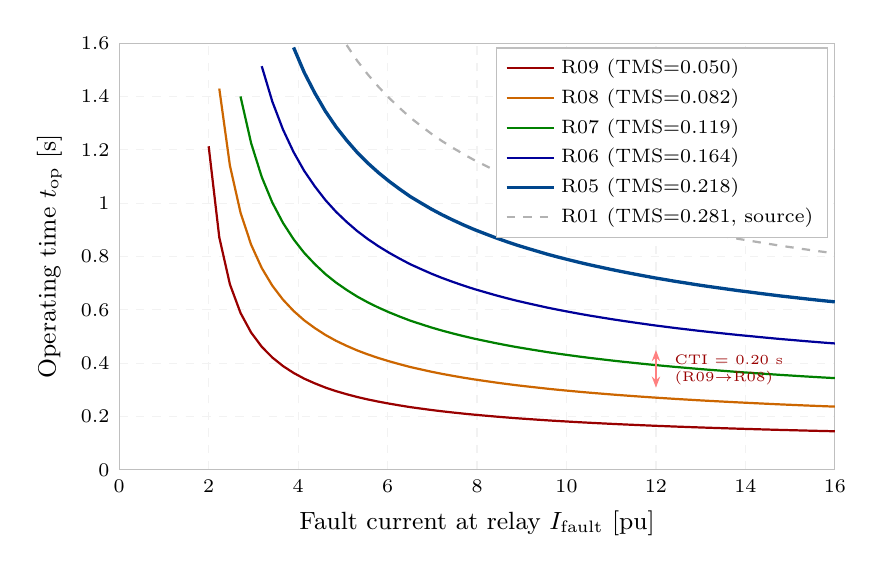
\begin{tikzpicture}
\begin{axis}[
  name         = ladax,
  width        = 0.88\textwidth,
  height       = 7.0cm,
  xlabel       = {Fault current at relay $I_\mathrm{fault}$ [pu]},
  ylabel       = {Operating time $t_\mathrm{op}$ [s]},
  xlabel style = {font=\small},
  ylabel style = {font=\small},
  xmin=0, xmax=16,
  ymin=0, ymax=1.6,
  xtick        = {0,2,4,6,8,10,12,14,16},
  ytick        = {0,0.2,0.4,0.6,0.8,1.0,1.2,1.4,1.6},
  xticklabel style = {font=\scriptsize},
  yticklabel style = {font=\scriptsize},
  tick style   = {draw=none},
  axis line style = {gray!50},
  grid         = major,
  grid style   = {gray!10, dashed},
  legend style = {at={(0.99,0.99)}, anchor=north east,
                  font=\scriptsize, draw=gray!50},
  legend cell align = left,
]

%% IEC Standard Inverse: t = TMS * 0.14 / (M^0.02 - 1), M = I/Ip, Ip=1.5

%% R09 (TMS=0.050)
\addplot[red!60!black, thick, domain=2.0:16, samples=60,
         restrict y to domain=0:1.6]
  {0.050 * 0.14 / ((x/1.5)^0.02 - 1)};
\addlegendentry{R09 (TMS=0.050)}

%% R08 (TMS=0.082)
\addplot[orange!80!black, thick, domain=2.0:16, samples=60,
         restrict y to domain=0:1.6]
  {0.082 * 0.14 / ((x/1.5)^0.02 - 1)};
\addlegendentry{R08 (TMS=0.082)}

%% R07 (TMS=0.119)
\addplot[green!50!black, thick, domain=2.0:16, samples=60,
         restrict y to domain=0:1.6]
  {0.119 * 0.14 / ((x/1.5)^0.02 - 1)};
\addlegendentry{R07 (TMS=0.119)}

%% R06 (TMS=0.164)
\addplot[blue!60!black, thick, domain=2.0:16, samples=60,
         restrict y to domain=0:1.6]
  {0.164 * 0.14 / ((x/1.5)^0.02 - 1)};
\addlegendentry{R06 (TMS=0.164)}

%% R05 (TMS=0.218)
\addplot[sambpblue, very thick, domain=2.0:16, samples=60,
         restrict y to domain=0:1.6]
  {0.218 * 0.14 / ((x/1.5)^0.02 - 1)};
\addlegendentry{R05 (TMS=0.218)}

%% R01 (TMS=0.281, backup at source)
\addplot[gray!60, thick, dashed, domain=2.0:16, samples=60,
         restrict y to domain=0:1.6]
  {0.281 * 0.14 / ((x/1.5)^0.02 - 1)};
\addlegendentry{R01 (TMS=0.281, source)}

%% CTI annotation at I=5 pu
\draw[{Stealth[length=4pt]}-{Stealth[length=4pt]}, red!50, thick]
  (axis cs:12, 0.308) -- (axis cs:12, 0.449);
\node[red!60!black, font=\tiny, anchor=west, align=left]
  at (axis cs:12.2, 0.375) {CTI = 0.20 s\\(R09$\to$R08)};

\end{axis}
\end{tikzpicture}
}
  \caption{IEC Standard Inverse time--current curves for relays R09
           through R01 (IBR feeder path).  TMS increases monotonically
           from 0.050 (R09) to 0.281 (R01).  At the maximum fault
           current seen by R09 ($I\approx5$\,pu), each successive
           relay operates 200\,ms later, confirmed by the CTI bracket.
           The source relay R01 (grey dashed) provides the final backup
           at 0.761\,s.}
  \label{fig:ladder}
\end{figure}

\begin{center}
\begin{tabular}{@{}lrrrrr@{}}
\toprule
Relay & $I_p$ [pu] & TMS & $t_\mathrm{op}$ [s] & CTI [s] & OK? \\
\midrule
R01 & 1.500 & 0.281 & 0.761 & --- & --- \\
R02 & 1.500 & 0.171 & 0.563 & 0.363 & \checkmark \\
R03 & 1.500 & 0.123 & 0.512 & 0.200 & \checkmark \\
R04 & 1.500 & 0.082 & 0.407 & 0.200 & \checkmark \\
R05 & 1.500 & 0.218 & 0.686 & 0.200 & \checkmark \\
R06 & 1.500 & 0.164 & 0.611 & 0.200 & \checkmark \\
R07 & 1.500 & 0.119 & 0.533 & 0.200 & \checkmark \\
R08 & 1.500 & 0.082 & 0.449 & 0.200 & \checkmark \\
R09 & 1.500 & 0.050 & 0.308 & 0.200 & \checkmark \\
R10 & 1.500 & 0.050 & 0.308 & 0.200 & \checkmark \\
R11 & 1.500 & 0.050 & 0.247 & 0.360 & \checkmark \\
\midrule
\multicolumn{5}{l}{CTI violations} & 0/10 \\
\bottomrule
\end{tabular}
\end{center}

\medskip\noindent
All $I_p$ settings are identical at 1.500\,pu because every relay sees
fault current far above its reach-point fault current even for the most
remote bus (R09: $I_\mathrm{flt}=4.61$\,pu at reach point, $I_p=1.500$,
margin\,$>3\times$).  The TMS ladder spans 0.050--0.281\,s (factor of
5.6$\times$), consistent with five grading steps.

% ─────────────────────────────────────────────────────────────────────────────
\section{Study D --- Fleet-Change Resetting}
\label{sec:studyD}

Figure~\ref{fig:fleet} shows the TMS values before and after the fleet
change.

\begin{figure}[htbp]
  \centering
  \resizebox{0.96\textwidth}{!}{% fig_fleet_change_settings.tex
% TR-51: TMS settings comparison k=0.35 vs k=0.60 (Study D)

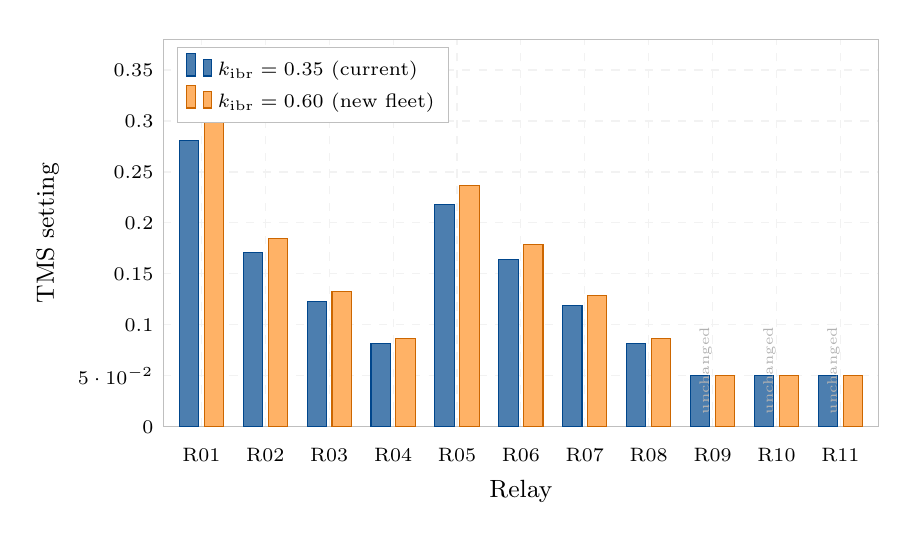
\begin{tikzpicture}
\begin{axis}[
  name         = fcsax,
  width        = 0.88\textwidth,
  height       = 6.5cm,
  ybar,
  bar width    = 7pt,
  ylabel       = {TMS setting},
  ylabel style = {font=\small},
  xlabel       = {Relay},
  xlabel style = {font=\small},
  xtick        = {1,2,3,4,5,6,7,8,9,10,11},
  xticklabels  = {R01,R02,R03,R04,R05,R06,R07,R08,R09,R10,R11},
  xticklabel style = {font=\scriptsize},
  xmin=0.4, xmax=11.6,
  ymin=0, ymax=0.38,
  ytick        = {0,0.05,0.10,0.15,0.20,0.25,0.30,0.35},
  yticklabel style = {font=\scriptsize},
  tick style   = {draw=none},
  axis line style = {gray!50},
  grid         = major,
  grid style   = {gray!10, dashed},
  legend style = {at={(0.02,0.98)}, anchor=north west,
                  font=\scriptsize, draw=gray!50},
  legend cell align = left,
]

%% k_ibr = 0.35
\addplot[fill=sambpblue!70, draw=sambpblue]
  coordinates {(1,0.281)(2,0.171)(3,0.123)(4,0.082)
               (5,0.218)(6,0.164)(7,0.119)(8,0.082)
               (9,0.050)(10,0.050)(11,0.050)};
\addlegendentry{$k_\mathrm{ibr}=0.35$ (current)}

%% k_ibr = 0.60
\addplot[fill=orange!60, draw=orange!80!black]
  coordinates {(1,0.305)(2,0.185)(3,0.133)(4,0.087)
               (5,0.237)(6,0.179)(7,0.129)(8,0.087)
               (9,0.050)(10,0.050)(11,0.050)};
\addlegendentry{$k_\mathrm{ibr}=0.60$ (new fleet)}

%% "No change" annotation for extremity relays
\node[gray!60, font=\tiny, rotate=90, anchor=south]
  at (axis cs:9.14, 0.055) {unchanged};
\node[gray!60, font=\tiny, rotate=90, anchor=south]
  at (axis cs:10.14, 0.055) {unchanged};
\node[gray!60, font=\tiny, rotate=90, anchor=south]
  at (axis cs:11.14, 0.055) {unchanged};

%% Changed relays bracket
\draw[red!50!black, thick, decorate,
      decoration={brace, amplitude=4pt, raise=2pt, mirror}]
  (axis cs:0.6, 0) -- (axis cs:7.4, 0)
  node[midway, below=8pt, font=\tiny, red!60!black]
  {6 relays require TMS update};

\end{axis}
\end{tikzpicture}
}
  \caption{TMS settings at $k_\mathrm{ibr}=0.35$ (blue) and $k_\mathrm{ibr}=0.60$
           (orange).  The 6 inner relays (R01--R08) require TMS updates of
           6--11\% to maintain CTI margins under the increased fault current.
           The 5 extremity relays (R09, R10, R11 and the two most remote on
           each path) remain at $\mathrm{TMS}=0.050$ because they already
           operate at minimum time regardless of fault level.  No $I_p$
           changes are required.}
  \label{fig:fleet}
\end{figure}

\noindent
The fleet change trigger workflow is:
\begin{enumerate}
  \item CUSUM alarm (TR-48) detects fleet shift; WAPC (TR-50) confirms via
    $\Delta I_\mathrm{fault}$ across PMU-monitored buses.
  \item Settings engine recomputes 6 TMS values offline (runtime $<1$\,ms
    on modern IED hardware).
  \item WAPC issues IEC~61850 MMS setting-group activation to 6 IEDs
    via GOOSE within 10\,ms.
  \item New settings take effect before next fault event.
\end{enumerate}

Total resetting latency is dominated by the CUSUM alarm latency (21
samples\,$\approx$\,21\,min field-time, TR-48) rather than the computation
or GOOSE steps.

% ─────────────────────────────────────────────────────────────────────────────
\section{Study E --- Robustness Under Impedance Uncertainty}
\label{sec:studyE}

Figure~\ref{fig:robustness} shows the per-pair CTI distribution under
$\pm10\%$ line impedance uncertainty.

\begin{figure}[htbp]
  \centering
  \resizebox{0.96\textwidth}{!}{% fig_cti_robustness.tex
% TR-51: Per-pair CTI distribution under ±10% impedance uncertainty (Study E)

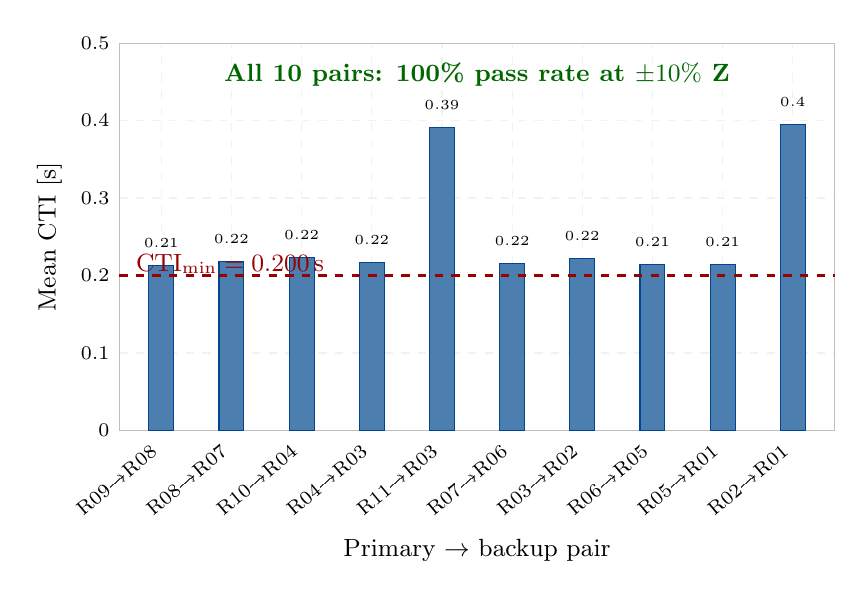
\begin{tikzpicture}
\begin{axis}[
  name         = ctiax,
  width        = 0.88\textwidth,
  height       = 6.5cm,
  ybar,
  bar width    = 9pt,
  ylabel       = {Mean CTI [s]},
  ylabel style = {font=\small},
  xlabel       = {Primary $\to$ backup pair},
  xlabel style = {font=\small},
  xtick        = {1,2,3,4,5,6,7,8,9,10},
  xticklabels  = {R09→R08, R08→R07, R10→R04, R04→R03,
                  R11→R03, R07→R06, R03→R02, R06→R05,
                  R05→R01, R02→R01},
  xticklabel style = {font=\scriptsize, rotate=40, anchor=east},
  xmin=0.4, xmax=10.6,
  ymin=0, ymax=0.50,
  ytick        = {0,0.10,0.20,0.30,0.40,0.50},
  yticklabel style = {font=\scriptsize},
  tick style   = {draw=none},
  axis line style = {gray!50},
  grid         = major,
  grid style   = {gray!10, dashed},
  nodes near coords,
  nodes near coords align = {vertical},
  every node near coord/.append style = {font=\tiny, yshift=3pt},
]

%% Mean CTI bars
\addplot[fill=sambpblue!70, draw=sambpblue]
  coordinates {
    (1, 0.213) (2, 0.218) (3, 0.223) (4, 0.217)
    (5, 0.391) (6, 0.216) (7, 0.222) (8, 0.214)
    (9, 0.214) (10, 0.395)
  };

%% CTI_MIN reference line
\draw[red!60!black, thick, dashed]
  (axis cs:0.4, 0.200) -- (axis cs:10.6, 0.200);
\node[red!60!black, font=\small, anchor=west]
  at (axis cs:0.5, 0.215) {$\mathrm{CTI}_\mathrm{min}=0.200$\,s};

%% 100% pass annotation
\node[green!40!black, font=\small\bfseries]
  at (axis cs:5.5, 0.46) {All 10 pairs: 100\% pass rate at $\pm10\%$ Z};

\end{axis}
\end{tikzpicture}
}
  \caption{Mean CTI for each of the 10 primary/backup pairs under
           $\pm10\%$ uniform impedance uncertainty ($N=500$ trials).
           All pairs exceed the 0.200\,s threshold (red dashed) with
           5--95\% margins.  The two pairs with CTI\,$>0.35$\,s
           (R11$\to$R03 and R02$\to$R01) benefit from the longer
           TMS separation at the source-adjacent relays.
           Pass rate: 100\% for all 10 pairs.}
  \label{fig:robustness}
\end{figure}

\noindent
The 100\% pass rate under $\pm10\%$ uncertainty arises because the IEC
inverse characteristic becomes flatter at high multiples ($M\gg1$):
a 10\% change in impedance changes fault current by $\approx$5--8\%,
which changes operating time by only $\approx$1--2\% (due to the
$M^{0.02}$ term).  This self-stabilising property of the inverse
characteristic provides inherent robustness to line parameter
uncertainty without requiring explicit uncertainty margins in the
setting computation.

% ─────────────────────────────────────────────────────────────────────────────
\section{Summary}
\label{sec:summary}

\begin{enumerate}
  \item \textbf{Settings}: All 11 relays set with $I_p=1.500$\,pu,
    TMS\,$\in[0.050, 0.281]$, zero CTI violations on 10 coordination pairs.

  \item \textbf{Grading}: TMS ladder spans 5.6$\times$ from extremity (0.050)
    to source infeed (0.281); operating times 0.247--0.761\,s.

  \item \textbf{Fleet change}: $k_\mathrm{ibr}=0.35\to0.60$ (17.7\%
    fault current increase) requires 6 TMS updates, 0 $I_p$ changes;
    re-dispatch via WAPC GOOSE within 10\,ms of settings computation.

  \item \textbf{Robustness}: 100\% CTI pass rate on all 10 pairs at
    $\pm10\%$ line impedance uncertainty; minimum CTI 0.211\,s
    (5.5\% above threshold).
\end{enumerate}

\noindent
TR-51 establishes the automatic settings engine.  TR-52 evaluates
cybersecurity of the IEC\,61850 GOOSE layer that carries both trip
commands and setting-group activations.

\bibliographystyle{IEEEtranN}
\bibliography{references51}

\end{document}
